% *******************************************************************************
% * Copyright (c) 2007 by Elexis
% * All rights reserved. This document and the accompanying materials
% * are made available under the terms of the Eclipse Public License v1.0
% * which accompanies this distribution, and is available at
% * http://www.eclipse.org/legal/epl-v10.html
% *
% * Contributors:
% *    G. Weirich - initial implementation
% *
% *  $Id: laborview.tex 4902 2009-01-03 10:47:34Z rgw_ch $
% *******************************************************************************
% !Mode:: "TeX:UTF-8" (encoding info for WinEdt)

\section{'View' - Résultats de laboratoire}
\index{Laboratoire - Introduction manuelle}
\index{Laboratoire - Visualiser résultats}
Elexis permet de visualiser en même temps des résultats internes ou externes automatiquement ou manuellement introduits .
La visualisation est défini par :
\begin{itemize}
  \item Un élément de laboratoire spécifique attribué au résultat
  \item Une date d'analyse
  \item Un patient auquel est attribué le résultat
\end{itemize}

L'élément de laboratoire définit comment et où le résultat de laboratoire doit être affiché et de quel type de valeurs de laboratoire il fait partie. La création des éléments de laboratoire n'est normalement nécessaire que lors de l'installation du logiciel ou si vous voulez intégrer des nouvelles analyses dans votre liste d'analyses.
La procédure précise est décrite sous configuration
 (page \pageref{config:labor}.

 %\usepackage{graphics} is needed for \includegraphics
\begin{figure}[htp]
\begin{center}
  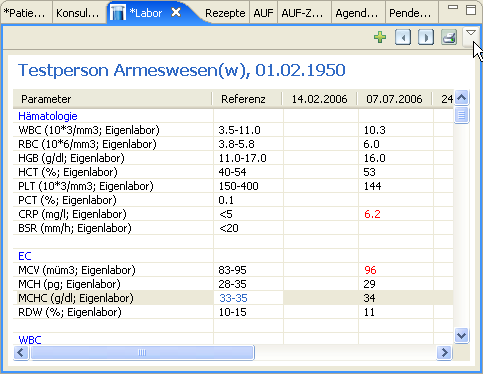
\includegraphics{images/labview}
  \caption{Labor-Anzeige}
  \label{fig:labview}
\end{center}
\end{figure}

\subsection{Introduction manuelle}
Pour introduire des résultats du laboratoire manuellement, il faut procéder comme suit :
\begin{itemize}
    \item S'il n'existe pas encore une colonne pour la date à laquelle vous faites les analyses, cliquez sur le signe Plus de couleur verte à droite en haut.
    \item Cliquez dans le champ où vous voulez introduire la valeur du labo. Introduisez la valeur et quittez par 'enter' ou la touche avec la flèche vers le bas.
\end{itemize}
Si un paramètre de laboratoire est numérique, et la valeur introduite se trouve hors du secteur de référence normal, le chiffre sera affiché en rouge. Vous pouvez activer ou désactiver manuellement ce réglage en cliquant sur le chiffre avec la touche droite de la souris et en activant ou désactivant le petit crochet devant l'indication  \glqq pathologique\grqq{}.

\subsection{Introduction automatisée}
\index{Laboratoire - Introduction automatisée}
Il va de soi qu'Elexis soit capable de introduire automatiquement les résultats de laboratoire. Pour ceci on utilise le 'view-menu' dans le coin supérieur droit :\\
\begin{wrapfigure}{r}{7cm}
    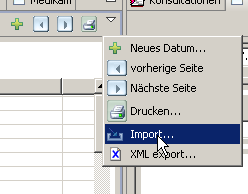
\includegraphics{images/labor6}
\end{wrapfigure}
Cliquez sur  \textit{importation} et choisissez dans la boîte de dialogue la source des valeurs de laboratoire à introduire. De quelles sources il s'agit dépend des Plugins existants pour l'importation des résultats de laboratoire.
Des appareils de laboratoire et différents laboratoires externes entrent en ligne de compte. Vous trouvez une liste actuelle de tous les Plugins d'importation de résultats de laboratoire existants sur
http://www.elexis.ch.

\subsection{Impression d'une feuille de labo}
Pour imprimer un feuille de laboratoire vous cliquez sur le symbole de l'imprimant qui se trouve à droite en haut. Ceci va créer un tableau dans le modèle de texte du système nommé \glqq feuille labo\grqq{}, qui contient une variable  [Valeurs de labo] (cf aussi \ref{textvorlagen}).

\section{Laboratoire Nouveau}
Cette 'View' permet d'afficher toutes les valeurs de laboratoire qui n'ont pas encore été marquées comme \glqq vu\grqq{} et permet en même temps de les marquer comme vues. (cf Fig. \ref{fig:labneu}).

\begin{figure}
  % Requires \usepackage{graphicx}
  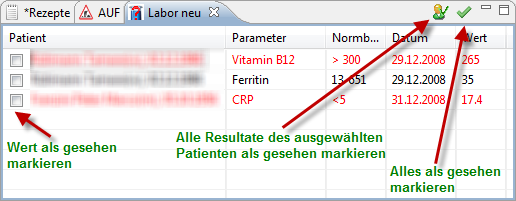
\includegraphics{images/labneu1}\\
  \caption{Anzeige neuer Laborwerte}\label{fig:labneu}
\end{figure}

Des valeurs à l'extérieur du secteur de référence sont représentées en rouge. Dans la boîte de contrôle à gauche, on peut marquer avec un crochet les résultats déjà vus. Après quelques temps, les résultats vus seront éliminés de la liste. (tant qu'ils ne sont pas encore éliminés, on peut éliminer la marquage 'vu' en cliquant à nouveau dessus). Des valeurs qui ont plus que 96 heures seront éliminées automatiquement de la liste.

En cliquant sur un résultat d'un patient on déclenche l'activation de la feuille labo de ce patient spécifique ( ... si jamais une View-Labo est ouverte). Pour marques les résultats comme vues on peut sélectionner soit seulement quelques valeurs soit tous les résultats du patient en question. 

Pour marquer des valeurs une à une ou dans l'ensemble comme 'vu', il faut avoir le droit : \textit{fichiers/patient/terminer labo}(cf \ref{sec:gruppen}, page\pageref{sec:gruppen}ff.)
